\documentclass{book}
\usepackage[utf8]{inputenc}
\usepackage[T1]{fontenc}
\usepackage[italian]{babel}
\usepackage{graphicx}
\usepackage{hyperref}
\usepackage{fancyhdr}
\fancyhf{}
\cfoot{\thepage}
\pagestyle{fancy}

\makeatletter
\renewcommand{\thesection}{\arabic{section}}
\renewcommand{\thechapter}{\arabic{chapter}}
\@addtoreset{section}{chapter}
\makeatother

\hypersetup{
  colorlinks=true,
  linkcolor=black,    % Colore dei collegamenti all'interno del documento
  urlcolor=black,     % Colore degli URL
  citecolor=black,    % Colore delle citazioni
  }
\begin{document}


\vspace*{\fill} 

\begin{center} 
    \textbf{Documentazione DNA-GymCraft} 
    \vskip 40pt
    Giuseppe Pio Sorrentino Antonio Albanese Marco Greco
\end{center}

\vspace*{\fill} 
\newpage
\begin{figure}
  \centering
  
\includegraphics[width=0.8\linewidth]{dipartimento.png}
  \captionof{\\LAURA TRIENNALE IN INFORMATICA UNIVERSITÀ DI SALERNO \\
  CORSO DI FONDAMENTI DI INTELLIGENZA ARTIFICIALE \\
  PROFESSORE FABIO PALOMBA}
\end{figure}


  
  
\includegraphics[width=0.8\linewidth]{LOGO.jpg}

\newline

Link repository GitHub: \href{https://github.com/Gmarco2706/DNAGYMCraft}{https://github.com/Gmarco2706/DNAGYMCraft}


\tableofcontents
\clearpage




\newpage
\section{Definizione del problema}
\subsection{Introduzione}
DNA-GymCraft è un algoritmo di intelligenza artificiale che nasce dall'idea di voler unire una passione di noi studenti con gli argomenti affrontati a lezione.\\ Questo algoritmo va incontro ai coach di una palestra perchè permette di creare una scheda di allenamento personalizzata a seconda del cliente basandosi su una serie di esercizi presi in input da un dataset contente circa 3000 esercizi. \\
\noindent
Questo algoritmo si basa molto anche sulle preferenze del cliente, esso infatti permette di modellare la scheda in base alle esigenze di quest'ultimo cercando di soddisfarlo il piu possibile utilizzando anche un sistema di feedback che permette di riprogrammare la scheda nel caso in cui il cliente non sia soddisfatto
Per poter realizzare questo algoritmo è stato utilizzato un algoritmo genetico
\subsection{Obiettivo}
L'Obiettivo del progetto è quello di realizzare una scheda che aiuti il coach a consegnarle per tutti i clienti della palestra in breve tempo e trovare la scheda perfetta per un cliente. La scheda deve essere quanto più bilanciata possibile, deve cercare di assegnare, in una scheda di sette esercizi, la giusta combinazione di esercizi per una determinata categoria (gambe, braccia e petto) comprendendo sempre un esercizio di streatching all'inizio e diversificando gli esercizi seguenti, privilegiando l'assegnazione di esercizi con attrezzi se il cliente  deve svolgere esercizi in palestra e in caso contrario assegnargli esercizi senza attrezzi per potergli permettere di svolgere la scheda assegnata senza problemi. Il feedback finale dell'utente si rivelerà poi molto importanto in quanto, in caso di feedback negativo, la scheda viene riformulata fin quando non riceverà un feedback positivo.
\section*{Tool utilizzati}
            \newline
            \noindent I tool da utilizzare per sviluppare il progetto sono:
            
                 Colab per l'implementazione dell'algoritmo
                  Python come linguaggio di programmazione
                  GitHub per condividere i lavori
                  Kaggle per trovare il dataset adatto al problema
                  Overleaf per la scrittura del documento del progetto
                Canva per la realizzazione della presentazione
             
\newpage
    \section{ Specifica PEAS} 
            \newline

                        \begin{tabular}{|p{1in}|p{4.1in}|} \hline 
                \multicolumn{2}{|p{2in}|}{\textbf{PEAS}} \\ \hline 
                \textbf{Performance} & La misura di performance dell'agente \`{e} la sua capacit\`{a} di massimizzare l'efficacia delle schede di allenamento generate in base alle preferenze dell'utente. \\ \hline 
                \textbf{Environment} & L'ambiente in cui opera il nostro agente riguarda l'ambito ginnico. L'ambiente \`{e}:\newline  \textbf{Dinamico} la dinamicità deriva dal fatto che l'agente (algoritmo genetico) interagisce con un ambiente in evoluzione, generando schede di allenamento in risposta alle preferenze e alle modifiche apportate dall'utente nel corso del tempo. L'ambiente è influenzato dalle scelte dell'utente, e l'agente si adatta continuamente per massimizzare le prestazioni delle schede di allenamento in base a tali preferenze e feedback.\newline  \textbf{Episodico }in quanto un'azione intrapresa dall'agente in un dato istante non \`{e} influenzata dall'azione effettuata precedentemente.\newline  \textbf{Totalmente osservabile }in quanto l'agente in ogni istante pu\`{o} avere una visione completa dell'ambiente in cui \`{e} calato.\newline   \textbf{Noto }in quanto abbiamo informazioni sulle dinamiche e le regole che guidano il processo di generazione delle schede di allenamento.\newline  \textbf{Singolo} in quanto l'ambiente prevede al proprio interno l'introduzione di un singolo agente.\newline Gli elementi dell'ambiente sono le schede di programmazione.\newline  \\ \hline 
                \textbf{Actuators} & L'agente agisce sull'ambiente tramite lo stream di output del nostro computer nel quale andr\`{a} generare una scheda di programmazione per una determinata persona \\ \hline 
                \textbf{Sensors} & L'agente percepir\'{a} l'ambiente tramite lo stream di input del nostro computer. \\ \hline 
            \end{tabular}
\newpage
\section{Analisi dei dati}
L'insieme degli esercizi è stato preso da un dataset su presente su Kaggle al seguente link \href{https://www.kaggle.com/datasets/niharika41298/gym-exercise-data}{https://www.kaggle.com/datasets/niharika41298/gym-exercise-data} contenente circa 3000 esercizi al suo interno e per ogni esercizio memorizza
\begin{itemize}
    \item titolo ovvero il nome dell'esercizio da svolgere
    \item descrizione ovvero una breve spiegazione dell'esercizio
    \item tipo di esercizio indica la tipologia di esercizio che viene svolto
    \item parte del corpo allenata
    \item equipaggiamento indica lo strumento da utilizzare per svolgere l'esercizio se l'esercizio ne necessita
    \item il livello di complessità per indicare quanto è complesso l'esercizio 
    \item il rating dell’esercizio, una valutazione media che viene data all'esercizio
    \item la descrizione del  rating, motivazione del voto assegnato
    
\end{itemize}
\newline

\section{Pulizia dei dati}

\begin{itemize}
 \item \subsection{ Rimozione colonne:}\newline
  
  La colonna \textbf{Descrizione} viene rimossa in quanto la maggior parte dei campi in quella colonna sono null, risulta inoltre essere inutile per l'algoritmo in quanto non va a influire sulla creazione della scheda \newline
  
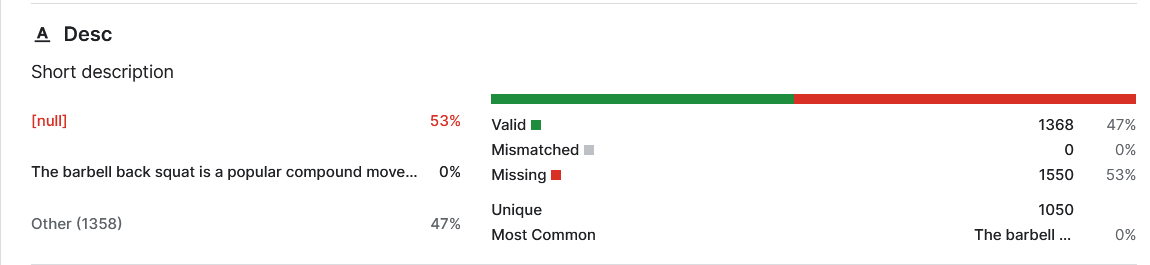
\includegraphics[width=1.0\linewidth]{info_descrizione.png}
\newpage

La colonna \textbf{Rating} viene rimossa anche in questo caso perche più della meta dei campi sono vuoti e essendo ogni esercizio indipendente dagli altri abbiamo deciso di non applicare tecniche di data imputation come la media in quanto basarci su rating di altri esercizi avrebbe potuto sopravvalutare o sottovalutare esercizi\newline

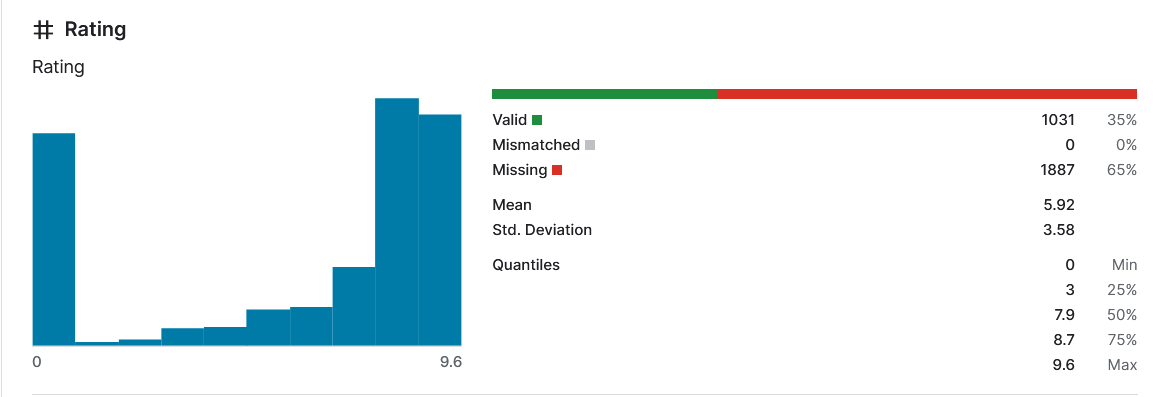
\includegraphics[width=1.0\linewidth]{info_rating.png}\newline
La colonna \textbf{RatingDesc} viene rimossa per un ragionamento analogo a quello della colonna descrizione e soprattuto perche eliminando la colonna Rating questa diventa inutile oltre a non essere influente e contenere per lo più valori nulli\newline

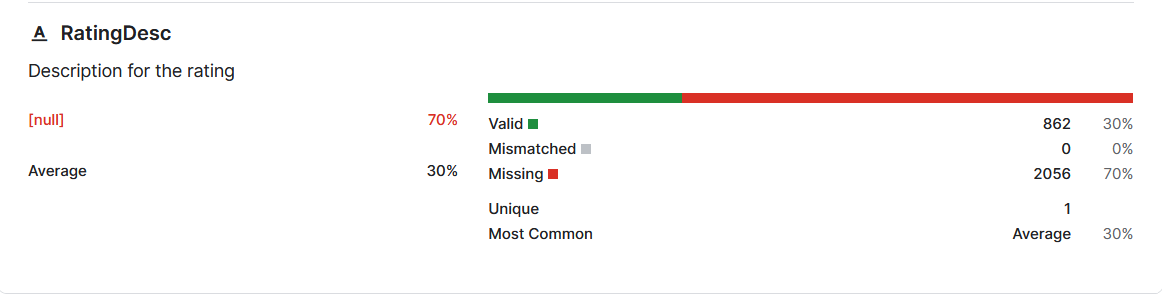
\includegraphics[width=1.0\linewidth]{info_ratingdesc.png}\newline

\item \subsection{ Rimozione righe:}\newline

Le righe contenenti campi vuoti nelle colonne di : titolo, tipo di esercizio, parte del corpo allenata, equipaggiamento necessario per svolgere l’esercizio e il livello di complessità vengono eliminate in quanto poche e essendo informazioni importanti non posso mancare\newline
\newpage
\item \subsection{ Riformattazione colonne:}\newline

Le colonne contenenti dati categorici sono state eliminate per lasciare spazio a valori binari che indicano l'appartenza di un esercizio a una determinata caratteristica. Per poter effettuare questa operazione abbiamo utilizzato la one hot encoding che scompone le varie categorie in colonne, se l'esercizio appartiene a una determinata categoria il valore corrispondente a quella colonna sarà 1 altrimenti 0 \newline


I vantaggi dell'utilizzo di una codifica one hot :\newline

Può migliorare le prestazioni del modello fornendo maggiori informazioni al modello sulle variabili categoriche.\\
Può aiutare a evitare il problema dell’ordinalità, che può verificarsi quando una variabile categorica ha un ordinamento naturale\newline

Gli svantaggi dell'utilizzo di una codifica one hot includono:\\

Può portare a una maggiore dimensionalità, poiché viene creata una colonna separata per ciascuna categoria nella variabile. Ciò può rendere il modello più complesso e lento da addestrare.\\
 Può portare a dati sparsi, poiché la maggior parte delle osservazioni avrà un valore pari a 0 nella maggior parte delle colonne.\newline

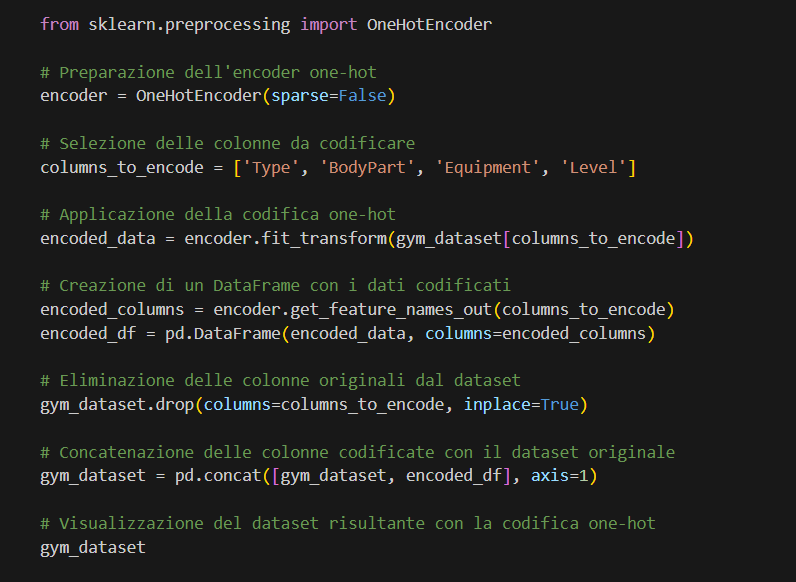
\includegraphics[width=1.0\linewidth]{onehotencoding.png}



\end{itemize}



\newpage
\section{Descrizione dell'Algoritmo}
\subsection{Rappresentazione degli individui}
L'output che l'algoritmo deve restituire è una scheda di allenamento contenente 7 esercizi, possiamo quindi rappresentare la scheda come una array di 7 elementi contenente per ogni cella il nome dell'esercizio da svolgere.\newline

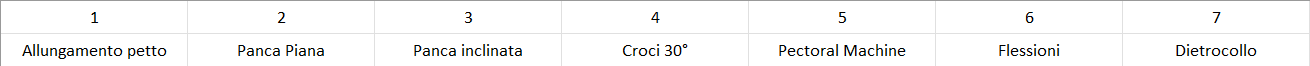
\includegraphics[width=1.0\linewidth]{Rappresentazione.png}

\subsection{Inizializzazione della popolazione}
La popolazione iniziale è generata pseudocasualmente attraverso una funzione che colloca al primo elemento della scheda un esercizio appartenente alla categoria di streatching  per poi riempire casualmente le altre celle basandosi sul tipo di allenamento scelto per quel giorno\newline

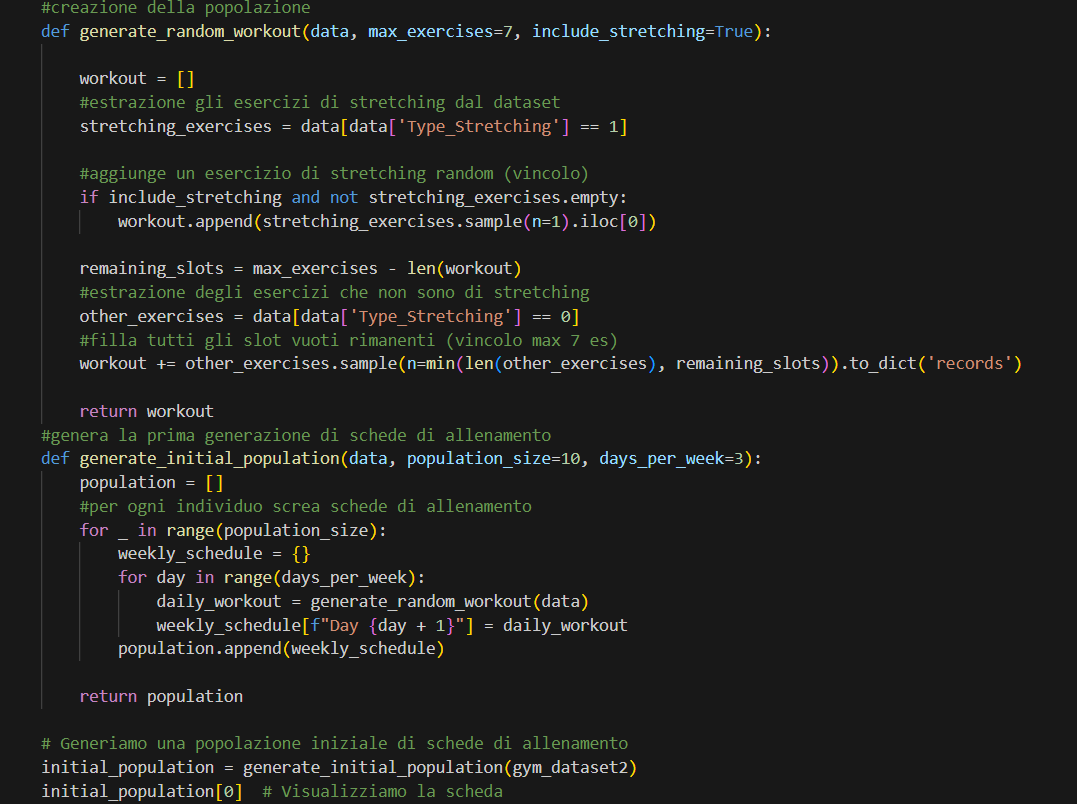
\includegraphics[width=1.0\linewidth]{CreazionePopolazione.png}
\subsection{Vincoli}
I vincoli imposti dal progetto sono i seguenti:
\begin{itemize}
    \item I giorni di allenamento sono 3
    \item Gli esercizi per ogni scheda sono 7
    \item Deve esserci un esercizio di streatching
\end{itemize}

 \subsection{Selezione degli individui}
  Per la selezione degli individui viene utilizzata la tecnica \textbf{K-Tournament Selection}, viene impostato il valore di k a 3 questo comporta che ad ogni selezione vengono casualmente scelti 3 individui dalla popolazione. Il miglior individuo (miglior valore di fitness) viene selezionato come genitore per la creazione della prossima generazione. E' stato scelto questo particolare algoritmo di selezione per evitare la problematica del super individuo e per la sua semplicità di implementazione e la possibilità da diminuire la diversità genetica o di diminuire la possibilità di una convergenza prematura.\newline

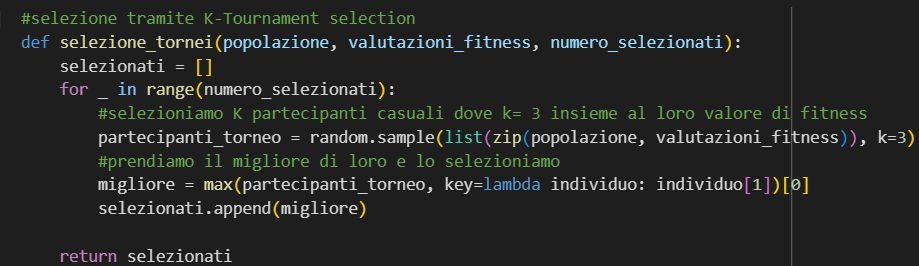
\includegraphics[width=1.0\linewidth]{Selection.png} 


  \subsection{Elitismo}
  viene applicato elitismo su due membri della popolazione, i due individui vengono scelti in base al loro valore di fitness. L'elitismo è stato applicato per stabilizzare l'algoritmo evitando ampie fluttuazioni tra i valori di fitness delle varie generazioni. \newline
  


  \subsection{Crossover}
  Viene Utilizzata la tecnica di \textbf{One-Point Crossover}, viene scelto un punto di crossover sulla lunghezza del genitore in modo randomico. Venegono combinati i due genitori in modo da creare un figlio con il corredo genetico costituito dalla zona prima del punto di crossover del genitore 1 unita alla zona dopo il punto di crossover del genitore2. La scelta è data dal fatto che il One-Point Crossover è molto efficace per problemi di ottimizzazioni semplici, inoltre ha un buon equilibrio tra esplorazione e integrità dei genitori.\newline

  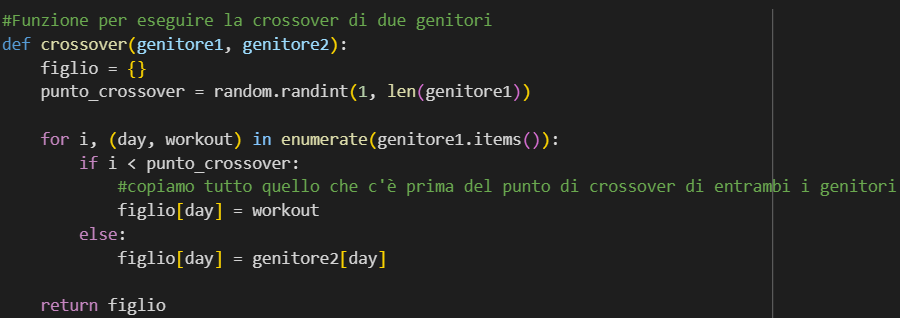
\includegraphics[width=1.0\linewidth]{Crossover.png} 
  
  \subsection{Mutazione}
  Per la mutazione è stata scelta una tecnica di \textbf{Random Resetting}, la randomizzazione è data dalla scelta di un numero casuale confrontato poi con un tasso di mutazione e dallo scambio di un esercizio casuale della scheda con uno casuale del dataset. Questa strategia di mutazione è stata scelta per via della varietà casuale che evita la convergenza prematura.\newline

  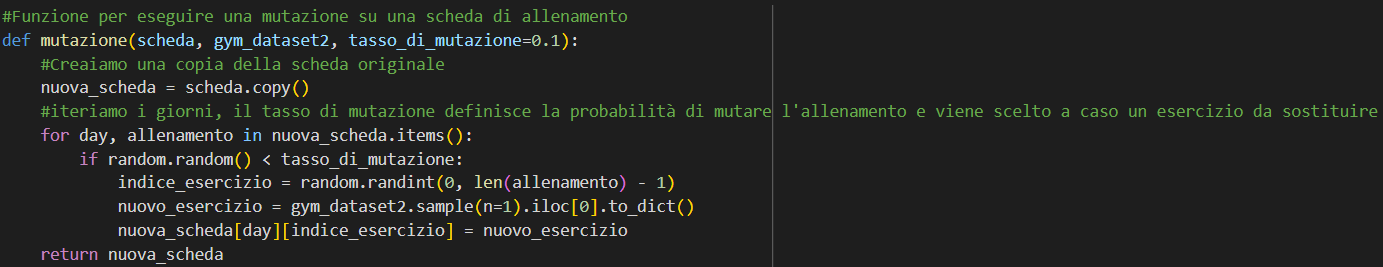
\includegraphics[width=1.0\linewidth]{Mutazione.png} 


  \subsection{Funzione di Fitness}
  La fitness di ogni scheda di allenamento generata è valutata tramite diversi criteri:
  \begin{itemize}
      \item \textbf{livello di abilità.}
            indica il livello di abilità selezionato in input dall'utente che può essere Principiante Intermedio Esperto, l'algoritmo in risposta all'input digitato preferirà esercizi del livello selezionato dall'utente.
      \item \textbf{varietà dei tipi di esercizi}
            indica il grado di varietà degli esercizi per evitare di eseguire sempre gli stessi esercizi nei vari giorni di allenamento,  di conseguenza l'algoritmo preferirà schede con tipi di esercizi diversi.
      \item \textbf{varietà dei gruppi muscolari}
            indica il grado di varietà dei gruppi muscolari allenati nei vari giorni della settimana per affaticare un determinato gruppo muscolare, di conseguenza l'algoritmo preferirà le schede che forniscono ampia varietà tra i gruppi muscolari.
      \item \textbf{luogo di allenamento}
            indica il luogo di allenamento selezionato in input dall'utente che può scegliere tra Casa e Palestra, per Casa l'algoritmo preferirà allenamenti senza strumenti o macchine viceversa se l'utente si allena in palestra gli verrà fornita una scheda con esercizi che sfruttano macchine o attrezzi.
      \item \textbf{Feedback}
            indica il feedback selezionato dall'utente dopo la stampa della prima scheda, l'utente può inserire tre feedback Troppo facile, Troppo intensa, Ottima. Di conseguenza l'algoritmo attribuirà dei punti in più o in meno alla scheda stampata in base al feedback dell'utente fornendo una scheda con delle modifiche.
  \end{itemize}
  Ogni criterio è stato pensato per contribuire al punteggio finale della fitness di ogni scheda di allenamento per soddisfare le esegenze di un utente andando a creare una scheda personalizzata secondo le sue esigenze, proprio a questo scopo è stato pensato un algoritmo genetico multiobiettivo .\newline


  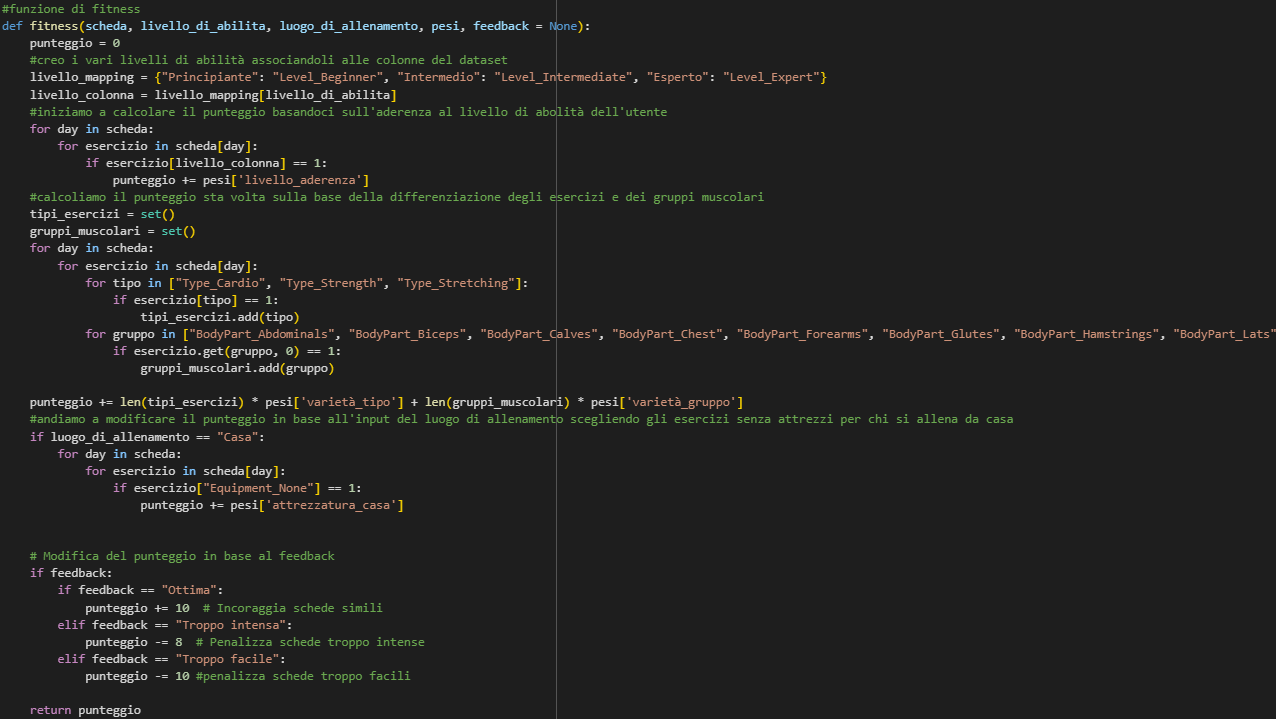
\includegraphics[width=1.0\linewidth]{Fitness.png}

  \subsection{Stopping Condition}
  La stopping condition scelta è quella di rendere fisso il numero di generazioni da creare tramite il parametro \textbf{numerogenerazioni}, questa scelta è stata fatta per tenere sotto controllo il tempo di esecuzione e il consumo di risorse dell'algoritmo.


  \section{Passi dell'algoritmo}
  Inizialmente viene chiesto all'utente di inserire in input il livello di abilità e il luogo dell'allenamento. Successivamente viene generata una popolazione iniziale di schede di allenamento, per ogni generazione avremo:
  \begin{enumerate}
      \item Calcolo della fitnes per ogni scheda della popolazione in base ai criteri forniti
      \item Selezione dei genitori per la creazione della next gen tramite K-Tournament Selection
      \item Creazione della nuova generazione tramite crossover One-Point e mutazione Random Resetting 
      \item Selezione della miglior scheda sulla base della fitness.
      \item Reiterazione su un numero fisso di generazioni e la ripetizione dei precedenti passi per ogni iterazione
      \item Viene inserito un input di feedback da parte dell'utente
      \item Seconda reiterazione con l'aggiunta del criterio inerente al feedback
  \end{enumerate}


  \subsection{Reiterazione}
  Dopo diverse esecuzioni abbiamo notato che l'algoritmo performi meglio se eseguito su più istanze, abbiamo notato quanto impatta il feedback sull'evoluzione della scheda. Si è notata anche una fluttuazione nei valori di fitness tra le varie generazioni per poi mostrare una convergenza verso la fine dell'esecuzione\newline
   


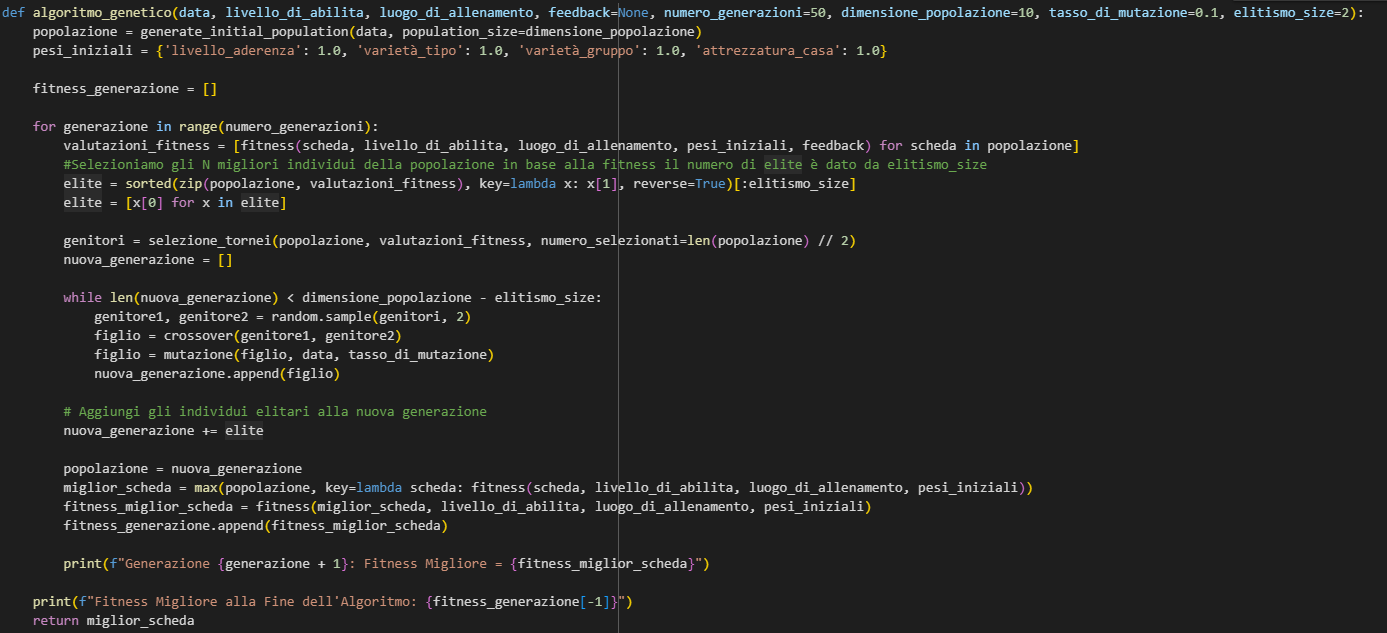
\includegraphics[width=1.0\linewidth]{Algoritmo.png}


  \section{Testing}
   Per la parte relativa al testing abbiamo inserito una funzione di testing che testasse l'algoritmo con tutte le combinazioni di input disponibili salvando i dati in un dataset

   \subsection{Numero di iterazioni}
   La fitness migliore non aumenta in modo significativo con il numero di iterazioni quindi un numero eccessivo potrebbe solo portare alla peggiorazione dell'efficienza dell'algoritmo.

   \subsection{durata delle iterazioni}
   La durata delle iterazioni rimane costante, da questo si evince che qualsiasi sia l'input inserito l'algoritmo è ottimo nel trovare una soluzione

   \subsection{Size della popolazione}
   Una popolazione troppo grande potrebbe rallentare l'intero algoritmo senza portare a miglioramenti significativi.

   \subsection{Dimensione dell'individuo}
   La dimensione sembra adeguata dato che l'algoritmo riesce a generare buone varietà di esercizi e si adatta bene al valore del feedback

   \section{Considerazioni finali}
    L'algoritmo mostra efficacia nel trovare buona soluzioni, più in generale l'algoritmo restituisce ottimi risultati per gli input di difficoltà intermedia ma ha difficoltà su l'input Esperto e su principiante e risponde bene al feedback dato dall'utente.\newline
    
    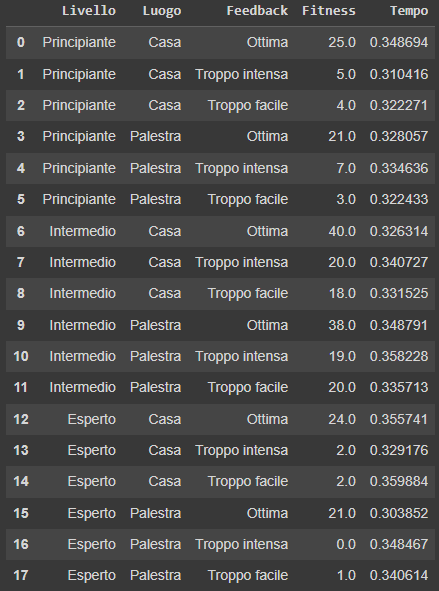
\includegraphics[width=1.0\linewidth]{test.png} 
\newpage
\section{Conclusioni}
L'implementazione di questo algoritmo è stata molto interessante, unire due delle nostre più grandi passioni ci ha permesso di lavorare in modo leggero cercando sempre di migliorare l'esecuzione con l'obiettivo di provare nella vita reale gli output forniti. Durante la fase di esecuzione abbiamo notato che l'algoritmo potrebbe generare errori su l'input Esperto e su principiante in quanto il dataset utilizzato presentava una grande variazione di esercizi di difficoltà intermedia e un pò meno dell'altro tipo di difficoltà. Siamo soddisfatti del lavoro svolto in quanto dall'inizio del corso non vedevamo l'ora di poter implementare algoritmi di intelligenza artificiale

\newpage
\textbf{Glossario}
\begin{itemize}
\item Dataset : Insieme di dati organizzati in forma relazionale. Ha una struttura tabellare, dove di solito ogni colonna rappresenta una variabile e ogni riga corrisponde a una osservazione.
\item Algoritmo Genetico : Procedura di alto livello (meta-euristica)
ispirata alla genetica per definire un algoritmo di ricerca. 
\item Specifica P.E.A.S. : Performance Environment Actuators Sensors, sintesi in una parola degli aspetti da prendere in considerazione nello studio dell’intelligenza Artificiale.
\item One Hot Encoding: ecnica che utilizziamo per rappresentare le variabili categoriali come valori numerici in un modello di machine learning
\item Data imputation: Insieme di tecniche che possono stimare il valore di dati mancanti sulla base dei dati disponibili oppure mitigare il problema dei dati mancanti
\item Selezione. Una copia di alcuni individui nella successiva generazione.
\item Crossover. Accoppiamento di individui (parents) per crearne di nuovi (offsprings), da aggiungere alla nuova generazione.
\item Mutazione. Una modifica casuale di alcune parti del corredo genetico.
\item Convergenza: Capacità di un GA di migliorare iterativamente le
soluzioni candidate verso il punto di ottimo
\item Funzione di fitness: funzione in grado di associare
un valore a ogni soluzione.
\item K-way tournament: K (< n) individui sono selezionati casualmente (formando il torneo) e il migliore tra questi K passa la selezione definitivamente. Si ripete finché non si arriva ad M tornei (e quindi M vincitori). Si possono avere selezioni ripetute.
\item Single Point: si seleziona un punto del patrimonio genetico dei genitori e si procede alla generazione di due figli tramite scambio di cromosomi.
\item Stopping Condition: Con quale criterio decidiamo di terminare l’evoluzione oppure proseguire
\item Elitismo : Operazione per la quale salviamo il migliore (o i migliori k) individuo e lo copiamo nella generazione successiva.

\end{itemize}



 

\end{document}

